% !TEX root = ../../../main.tex
% 来源：中学数学实验教材·第三册（高中数学）
% 章节：任意角的三角函数 / 弧和角的概念及其度量
% 原始文件：6.tex，行 270-285
% 类型：tikz
% ---
    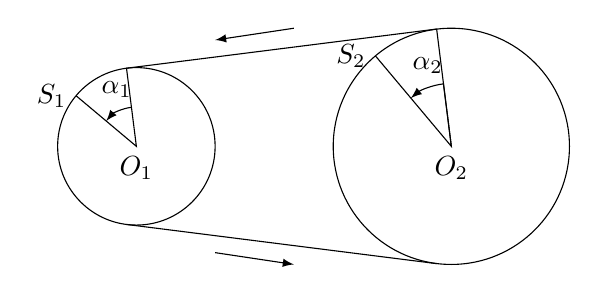
\begin{tikzpicture}[>=latex]
\draw (0,0) circle (1);
\draw (4,0) circle (1.5);
\node at  (0,0) [below]{$O_1$};
\node at  (4,0) [below]{$O_2$};
\draw (140:1)node[left]{$S_1$}--(0,0)--(97.2:1)--+(7.2:3.97)--(4,0)--+(130:1.5)node[left]{$S_2$};
\draw (-97.2:1)--+(-7.2:3.97);
\draw[->] (97.2:.5) arc (97.2:140:.5);
\draw[->] (4,0)--+(97.2:.8) arc (97.2:130:.8);
\node at (-.25,.5)[above]{$\alpha_1$};
\node at (4-.3,.8)[above]{$\alpha_2$};

\draw[<-]  (1,1.35)--(2,1.5);
\draw [->] (1,-1.35)--(2,-1.5);

    \end{tikzpicture}
